% REV01 Fri 25 Jun 2021 22:08:26 WIB
% START Tue 04 May 2021 13:55:16 WIB

\chapter{THE GOLDEN DUSTMAN FALLS INTO WORSE COMPANY}

It had come to pass that Mr Silas Wegg now rarely attended the minion of
fortune and the worm of the hour, at his (the worm’s and minion’s) own
house, but lay under general instructions to await him within a certain
margin of hours at the Bower. Mr Wegg took this arrangement in great
dudgeon, because the appointed hours were evening hours, and those he
considered precious to the progress of the friendly move. But it was
quite in character, he bitterly remarked to Mr Venus, that the upstart
who had trampled on those eminent creatures, Miss Elizabeth, Master
George, Aunt Jane, and Uncle Parker, should oppress his literary man.

The Roman Empire having worked out its destruction, Mr Boffin next
appeared in a cab with Rollin’s Ancient History, which valuable work
being found to possess lethargic properties, broke down, at about the
period when the whole of the army of Alexander the Macedonian (at that
time about forty thousand strong) burst into tears simultaneously, on
his being taken with a shivering fit after bathing. The Wars of the
Jews, likewise languishing under Mr Wegg’s generalship, Mr Boffin
arrived in another cab with Plutarch: whose Lives he found in the sequel
extremely entertaining, though he hoped Plutarch might not expect him to
believe them all. What to believe, in the course of his reading, was Mr
Boffin’s chief literary difficulty indeed; for some time he was divided
in his mind between half, all, or none; at length, when he decided, as a
moderate man, to compound with half, the question still remained, which
half? And that stumbling-block he never got over.

One evening, when Silas Wegg had grown accustomed to the arrival of
his patron in a cab, accompanied by some profane historian charged with
unutterable names of incomprehensible peoples, of impossible descent,
waging wars any number of years and syllables long, and carrying
illimitable hosts and riches about, with the greatest ease, beyond the
confines of geography--one evening the usual time passed by, and no
patron appeared. After half an hour’s grace, Mr Wegg proceeded to the
outer gate, and there executed a whistle, conveying to Mr Venus,
if perchance within hearing, the tidings of his being at home and
disengaged. Forth from the shelter of a neighbouring wall, Mr Venus then
emerged.

‘Brother in arms,’ said Mr Wegg, in excellent spirits, ‘welcome!’

In return, Mr Venus gave him a rather dry good evening.

‘Walk in, brother,’ said Silas, clapping him on the shoulder, ‘and take
your seat in my chimley corner; for what says the ballad?

\begin{verbatim}
     "No malice to dread, sir,
     And no falsehood to fear,
     But truth to delight me, Mr Venus,
     And I forgot what to cheer.
     Li toddle de om dee.
     And something to guide,
     My ain fireside, sir,
     My ain fireside.”’
\end{verbatim}

With this quotation (depending for its neatness rather on the spirit
than the words), Mr Wegg conducted his guest to his hearth.

‘And you come, brother,’ said Mr Wegg, in a hospitable glow, ‘you come
like I don’t know what--exactly like it--I shouldn’t know you from
it--shedding a halo all around you.’

‘What kind of halo?’ asked Mr Venus.

‘’Ope sir,’ replied Silas. ‘That’s YOUR halo.’

Mr Venus appeared doubtful on the point, and looked rather
discontentedly at the fire.

‘We’ll devote the evening, brother,’ exclaimed Wegg, ‘to prosecute our
friendly move. And arterwards, crushing a flowing wine-cup--which I
allude to brewing rum and water--we’ll pledge one another. For what says
the Poet?

\begin{verbatim}
     "And you needn’t Mr Venus be your black bottle,
     For surely I’ll be mine,
     And we’ll take a glass with a slice of lemon in it to which
     you’re partial,
     For auld lang syne.”’
\end{verbatim}

This flow of quotation and hospitality in Wegg indicated his observation
of some little querulousness on the part of Venus.

‘Why, as to the friendly move,’ observed the last-named gentleman,
rubbing his knees peevishly, ‘one of my objections to it is, that it
DON’T move.’

‘Rome, brother,’ returned Wegg: ‘a city which (it may not be generally
known) originated in twins and a wolf; and ended in Imperial marble:
wasn’t built in a day.’

‘Did I say it was?’ asked Venus.

‘No, you did not, brother. Well-inquired.’

‘But I do say,’ proceeded Venus, ‘that I am taken from among my trophies
of anatomy, am called upon to exchange my human warious for mere
coal-ashes warious, and nothing comes of it. I think I must give up.’

‘No, sir!’ remonstrated Wegg, enthusiastically. ‘No, Sir!

\begin{verbatim}
     "Charge, Chester, charge,
     On, Mr Venus, on!”
\end{verbatim}

Never say die, sir! A man of your mark!’

‘It’s not so much saying it that I object to,’ returned Mr Venus, ‘as
doing it. And having got to do it whether or no, I can’t afford to waste
my time on groping for nothing in cinders.’

‘But think how little time you have given to the move, sir, after all,’
urged Wegg. ‘Add the evenings so occupied together, and what do they
come to? And you, sir, harmonizer with myself in opinions, views, and
feelings, you with the patience to fit together on wires the whole
framework of society--I allude to the human skelinton--you to give in so
soon!’

‘I don’t like it,’ returned Mr Venus moodily, as he put his head between
his knees and stuck up his dusty hair. ‘And there’s no encouragement to
go on.’

‘Not them Mounds without,’ said Mr Wegg, extending his right hand with
an air of solemn reasoning, ‘encouragement? Not them Mounds now looking
down upon us?’

‘They’re too big,’ grumbled Venus. ‘What’s a scratch here and a scrape
there, a poke in this place and a dig in the other, to them. Besides;
what have we found?’

‘What HAVE we found?’ cried Wegg, delighted to be able to acquiesce.
‘Ah! There I grant you, comrade. Nothing. But on the contrary, comrade,
what MAY we find? There you’ll grant me. Anything.’

‘I don’t like it,’ pettishly returned Venus as before. ‘I came into
it without enough consideration. And besides again. Isn’t your own Mr
Boffin well acquainted with the Mounds? And wasn’t he well acquainted
with the deceased and his ways? And has he ever showed any expectation
of finding anything?’

At that moment wheels were heard.

‘Now, I should be loth,’ said Mr Wegg, with an air of patient injury,
‘to think so ill of him as to suppose him capable of coming at this time
of night. And yet it sounds like him.’

A ring at the yard bell.

‘It is him,’ said Mr Wegg, ‘and he is capable of it. I am sorry, because
I could have wished to keep up a little lingering fragment of respect
for him.’

Here Mr Boffin was heard lustily calling at the yard gate, ‘Halloa!
Wegg! Halloa!’

‘Keep your seat, Mr Venus,’ said Wegg. ‘He may not stop.’ And then
called out, ‘Halloa, sir! Halloa! I’m with you directly, sir! Half a
minute, Mr Boffin. Coming, sir, as fast as my leg will bring me!’ And
so with a show of much cheerful alacrity stumped out to the gate with
a light, and there, through the window of a cab, descried Mr Boffin
inside, blocked up with books.

‘Here! lend a hand, Wegg,’ said Mr Boffin excitedly, ‘I can’t get out
till the way is cleared for me. This is the Annual Register, Wegg, in a
cab-full of wollumes. Do you know him?’

‘Know the Animal Register, sir?’ returned the Impostor, who had caught
the name imperfectly. ‘For a trifling wager, I think I could find any
Animal in him, blindfold, Mr Boffin.’

‘And here’s Kirby’s Wonderful Museum,’ said Mr Boffin, ‘and Caulfield’s
Characters, and Wilson’s. Such Characters, Wegg, such Characters! I must
have one or two of the best of ‘em to-night. It’s amazing what places
they used to put the guineas in, wrapped up in rags. Catch hold of that
pile of wollumes, Wegg, or it’ll bulge out and burst into the mud. Is
there anyone about, to help?’

‘There’s a friend of mine, sir, that had the intention of spending
the evening with me when I gave you up--much against my will--for the
night.’

‘Call him out,’ cried Mr Boffin in a bustle; ‘get him to bear a hand.
Don’t drop that one under your arm. It’s Dancer. Him and his sister made
pies of a dead sheep they found when they were out a walking. Where’s
your friend? Oh, here’s your friend. Would you be so good as help Wegg
and myself with these books? But don’t take Jemmy Taylor of Southwark,
nor yet Jemmy Wood of Gloucester. These are the two Jemmys. I’ll carry
them myself.’

Not ceasing to talk and bustle, in a state of great excitement, Mr
Boffin directed the removal and arrangement of the books, appearing
to be in some sort beside himself until they were all deposited on the
floor, and the cab was dismissed.

‘There!’ said Mr Boffin, gloating over them. ‘There they are, like the
four-and-twenty fiddlers--all of a row. Get on your spectacles, Wegg;
I know where to find the best of ‘em, and we’ll have a taste at once of
what we have got before us. What’s your friend’s name?’

Mr Wegg presented his friend as Mr Venus.

‘Eh?’ cried Mr Boffin, catching at the name. ‘Of Clerkenwell?’

‘Of Clerkenwell, sir,’ said Mr Venus.

‘Why, I’ve heard of you,’ cried Mr Boffin, ‘I heard of you in the
old man’s time. You knew him. Did you ever buy anything of him?’ With
piercing eagerness.

‘No, sir,’ returned Venus.

‘But he showed you things; didn’t he?’

Mr Venus, with a glance at his friend, replied in the affirmative.

‘What did he show you?’ asked Mr Boffin, putting his hands behind him,
and eagerly advancing his head. ‘Did he show you boxes, little cabinets,
pocket-books, parcels, anything locked or sealed, anything tied up?’

Mr Venus shook his head.

‘Are you a judge of china?’

Mr Venus again shook his head.

‘Because if he had ever showed you a teapot, I should be glad to know of
it,’ said Mr Boffin. And then, with his right hand at his lips, repeated
thoughtfully, ‘a Teapot, a Teapot’, and glanced over the books on the
floor, as if he knew there was something interesting connected with a
teapot, somewhere among them.

Mr Wegg and Mr Venus looked at one another wonderingly: and Mr Wegg, in
fitting on his spectacles, opened his eyes wide, over their rims, and
tapped the side of his nose: as an admonition to Venus to keep himself
generally wide awake.

‘A Teapot,’ repeated Mr Boffin, continuing to muse and survey the books;
‘a Teapot, a Teapot. Are you ready, Wegg?’

‘I am at your service, sir,’ replied that gentleman, taking his usual
seat on the usual settle, and poking his wooden leg under the table
before it. ‘Mr Venus, would you make yourself useful, and take a seat
beside me, sir, for the conveniency of snuffing the candles?’

Venus complying with the invitation while it was yet being given, Silas
pegged at him with his wooden leg, to call his particular attention to
Mr Boffin standing musing before the fire, in the space between the two
settles.

‘Hem! Ahem!’ coughed Mr Wegg to attract his employer’s attention. ‘Would
you wish to commence with an Animal, sir--from the Register?’

‘No,’ said Mr Boffin, ‘no, Wegg.’ With that, producing a little book
from his breast-pocket, he handed it with great care to the literary
gentlemen, and inquired, ‘What do you call that, Wegg?’

‘This, sir,’ replied Silas, adjusting his spectacles, and referring to
the title-page, ‘is Merryweather’s Lives and Anecdotes of Misers. Mr
Venus, would you make yourself useful and draw the candles a little
nearer, sir?’ This to have a special opportunity of bestowing a stare
upon his comrade.

‘Which of ‘em have you got in that lot?’ asked Mr Boffin. ‘Can you find
out pretty easy?’

‘Well, sir,’ replied Silas, turning to the table of contents and slowly
fluttering the leaves of the book, ‘I should say they must be pretty
well all here, sir; here’s a large assortment, sir; my eye catches John
Overs, sir, John Little, sir, Dick Jarrel, John Elwes, the Reverend Mr
Jones of Blewbury, Vulture Hopkins, Daniel Dancer--’

‘Give us Dancer, Wegg,’ said Mr Boffin.

With another stare at his comrade, Silas sought and found the place.

‘Page a hundred and nine, Mr Boffin. Chapter eight. Contents of chapter,
“His birth and estate. His garments and outward appearance. Miss Dancer
and her feminine graces. The Miser’s Mansion. The finding of a treasure.
The Story of the Mutton Pies. A Miser’s Idea of Death. Bob, the Miser’s
cur. Griffiths and his Master. How to turn a penny. A substitute for a
Fire. The Advantages of keeping a Snuff-box. The Miser dies without a
Shirt. The Treasures of a Dunghill--“’

‘Eh? What’s that?’ demanded Mr Boffin.

‘“The Treasures,” sir,’ repeated Silas, reading very distinctly, ‘“of a
Dunghill.” Mr Venus, sir, would you obleege with the snuffers?’ This, to
secure attention to his adding with his lips only, ‘Mounds!’

Mr Boffin drew an arm-chair into the space where he stood, and said,
seating himself and slyly rubbing his hands:

‘Give us Dancer.’

Mr Wegg pursued the biography of that eminent man through its various
phases of avarice and dirt, through Miss Dancer’s death on a sick
regimen of cold dumpling, and through Mr Dancer’s keeping his rags
together with a hayband, and warming his dinner by sitting upon it, down
to the consolatory incident of his dying naked in a sack. After which he
read on as follows:

‘“The house, or rather the heap of ruins, in which Mr Dancer lived, and
which at his death devolved to the right of Captain Holmes, was a most
miserable, decayed building, for it had not been repaired for more than
half a century.”’

(Here Mr Wegg eyes his comrade and the room in which they sat: which had
not been repaired for a long time.)

‘“But though poor in external structure, the ruinous fabric was very
rich in the interior. It took many weeks to explore its whole contents;
and Captain Holmes found it a very agreeable task to dive into the
miser’s secret hoards.”’

(Here Mr Wegg repeated ‘secret hoards’, and pegged his comrade again.)

‘“One of Mr Dancer’s richest escretoires was found to be a dungheap in
the cowhouse; a sum but little short of two thousand five hundred
pounds was contained in this rich piece of manure; and in an old jacket,
carefully tied, and strongly nailed down to the manger, in bank notes
and gold were found five hundred pounds more.”’

(Here Mr Wegg’s wooden leg started forward under the table, and slowly
elevated itself as he read on.)

‘“Several bowls were discovered filled with guineas and half-guineas;
and at different times on searching the corners of the house they found
various parcels of bank notes. Some were crammed into the crevices of
the wall”’;

(Here Mr Venus looked at the wall.)

‘“Bundles were hid under the cushions and covers of the chairs”’;

(Here Mr Venus looked under himself on the settle.)

‘“Some were reposing snugly at the back of the drawers; and notes
amounting to six hundred pounds were found neatly doubled up in the
inside of an old teapot. In the stable the Captain found jugs full of
old dollars and shillings. The chimney was not left unsearched, and paid
very well for the trouble; for in nineteen different holes, all filled
with soot, were found various sums of money, amounting together to more
than two hundred pounds.”’

On the way to this crisis Mr Wegg’s wooden leg had gradually elevated
itself more and more, and he had nudged Mr Venus with his opposite
elbow deeper and deeper, until at length the preservation of his balance
became incompatible with the two actions, and he now dropped over
sideways upon that gentleman, squeezing him against the settle’s edge.
Nor did either of the two, for some few seconds, make any effort to
recover himself; both remaining in a kind of pecuniary swoon.

But the sight of Mr Boffin sitting in the arm-chair hugging himself,
with his eyes upon the fire, acted as a restorative. Counterfeiting a
sneeze to cover their movements, Mr Wegg, with a spasmodic ‘Tish-ho!’
pulled himself and Mr Venus up in a masterly manner.

‘Let’s have some more,’ said Mr Boffin, hungrily.

‘John Elwes is the next, sir. Is it your pleasure to take John Elwes?’

‘Ah!’ said Mr Boffin. ‘Let’s hear what John did.’

He did not appear to have hidden anything, so went off rather flatly.
But an exemplary lady named Wilcocks, who had stowed away gold and
silver in a pickle-pot in a clock-case, a canister-full of treasure in
a hole under her stairs, and a quantity of money in an old rat-trap,
revived the interest. To her succeeded another lady, claiming to be a
pauper, whose wealth was found wrapped up in little scraps of paper and
old rag. To her, another lady, apple-woman by trade, who had saved a
fortune of ten thousand pounds and hidden it ‘here and there, in cracks
and corners, behind bricks and under the flooring.’ To her, a French
gentleman, who had crammed up his chimney, rather to the detriment
of its drawing powers, ‘a leather valise, containing twenty thousand
francs, gold coins, and a large quantity of precious stones,’ as
discovered by a chimneysweep after his death. By these steps Mr Wegg
arrived at a concluding instance of the human Magpie:

‘Many years ago, there lived at Cambridge a miserly old couple of the
name of Jardine: they had two sons: the father was a perfect miser, and
at his death one thousand guineas were discovered secreted in his bed.
The two sons grew up as parsimonious as their sire. When about twenty
years of age, they commenced business at Cambridge as drapers, and
they continued there until their death. The establishment of the Messrs
Jardine was the most dirty of all the shops in Cambridge. Customers
seldom went in to purchase, except perhaps out of curiosity. The
brothers were most disreputable-looking beings; for, although surrounded
with gay apparel as their staple in trade, they wore the most filthy
rags themselves. It is said that they had no bed, and, to save the
expense of one, always slept on a bundle of packing-cloths under the
counter. In their housekeeping they were penurious in the extreme. A
joint of meat did not grace their board for twenty years. Yet when the
first of the brothers died, the other, much to his surprise, found large
sums of money which had been secreted even from him.’

‘There!’ cried Mr Boffin. ‘Even from him, you see! There was only two of
‘em, and yet one of ‘em hid from the other.’

Mr Venus, who since his introduction to the French gentleman, had been
stooping to peer up the chimney, had his attention recalled by the last
sentence, and took the liberty of repeating it.

‘Do you like it?’ asked Mr Boffin, turning suddenly.

‘I beg your pardon, sir?’

‘Do you like what Wegg’s been a-reading?’

Mr Venus answered that he found it extremely interesting.

‘Then come again,’ said Mr Boffin, ‘and hear some more. Come when you
like; come the day after to-morrow, half an hour sooner. There’s plenty
more; there’s no end to it.’

Mr Venus expressed his acknowledgments and accepted the invitation.

‘It’s wonderful what’s been hid, at one time and another,’ said Mr
Boffin, ruminating; ‘truly wonderful.’

‘Meaning sir,’ observed Wegg, with a propitiatory face to draw him out,
and with another peg at his friend and brother, ‘in the way of money?’

‘Money,’ said Mr Boffin. ‘Ah! And papers.’

Mr Wegg, in a languid transport, again dropped over on Mr Venus, and
again recovering himself, masked his emotions with a sneeze.

‘Tish-ho! Did you say papers too, sir? Been hidden, sir?’

‘Hidden and forgot,’ said Mr Boffin. ‘Why the bookseller that sold me
the Wonderful Museum--where’s the Wonderful Museum?’ He was on his knees
on the floor in a moment, groping eagerly among the books.

‘Can I assist you, sir?’ asked Wegg.

‘No, I have got it; here it is,’ said Mr Boffin, dusting it with the
sleeve of his coat. ‘Wollume four. I know it was the fourth wollume,
that the bookseller read it to me out of. Look for it, Wegg.’

Silas took the book and turned the leaves.

‘Remarkable petrefaction, sir?’

‘No, that’s not it,’ said Mr Boffin. ‘It can’t have been a
petrefaction.’

‘Memoirs of General John Reid, commonly called The Walking Rushlight,
sir? With portrait?’

‘No, nor yet him,’ said Mr Boffin.

‘Remarkable case of a person who swallowed a crown-piece, sir?’

‘To hide it?’ asked Mr Boffin.

‘Why, no, sir,’ replied Wegg, consulting the text, ‘it appears to have
been done by accident. Oh! This next must be it. “Singular discovery of
a will, lost twenty-one years.”’

‘That’s it!’ cried Mr Boffin. ‘Read that.’

‘“A most extraordinary case,”’ read Silas Wegg aloud, ‘“was tried at
the last Maryborough assizes in Ireland. It was briefly this. Robert
Baldwin, in March 1782, made his will, in which he devised the lands now
in question, to the children of his youngest son; soon after which his
faculties failed him, and he became altogether childish and died, above
eighty years old. The defendant, the eldest son, immediately afterwards
gave out that his father had destroyed the will; and no will being
found, he entered into possession of the lands in question, and so
matters remained for twenty-one years, the whole family during all
that time believing that the father had died without a will. But after
twenty-one years the defendant’s wife died, and he very soon afterwards,
at the age of seventy-eight, married a very young woman: which caused
some anxiety to his two sons, whose poignant expressions of this feeling
so exasperated their father, that he in his resentment executed a will
to disinherit his eldest son, and in his fit of anger showed it to his
second son, who instantly determined to get at it, and destroy it, in
order to preserve the property to his brother. With this view, he broke
open his father’s desk, where he found--not his father’s will which he
sought after, but the will of his grandfather, which was then altogether
forgotten in the family.”’

‘There!’ said Mr Boffin. ‘See what men put away and forget, or mean to
destroy, and don’t!’ He then added in a slow tone, ‘As--ton--ish--ing!’
And as he rolled his eyes all round the room, Wegg and Venus likewise
rolled their eyes all round the room. And then Wegg, singly, fixed his
eyes on Mr Boffin looking at the fire again; as if he had a mind to
spring upon him and demand his thoughts or his life.

‘However, time’s up for to-night,’ said Mr Boffin, waving his hand after
a silence. ‘More, the day after to-morrow. Range the books upon the
shelves, Wegg. I dare say Mr Venus will be so kind as help you.’

While speaking, he thrust his hand into the breast of his outer coat,
and struggled with some object there that was too large to be got out
easily. What was the stupefaction of the friendly movers when this
object at last emerging, proved to be a much-dilapidated dark lantern!

Without at all noticing the effect produced by this little instrument,
Mr Boffin stood it on his knee, and, producing a box of matches,
deliberately lighted the candle in the lantern, blew out the kindled
match, and cast the end into the fire. ‘I’m going, Wegg,’ he then
announced, ‘to take a turn about the place and round the yard. I don’t
want you. Me and this same lantern have taken hundreds--thousands--of
such turns in our time together.’

‘But I couldn’t think, sir--not on any account, I couldn’t,’--Wegg was
politely beginning, when Mr Boffin, who had risen and was going towards
the door, stopped:

‘I have told you that I don’t want you, Wegg.’

Wegg looked intelligently thoughtful, as if that had not occurred to his
mind until he now brought it to bear on the circumstance. He had nothing
for it but to let Mr Boffin go out and shut the door behind him. But,
the instant he was on the other side of it, Wegg clutched Venus
with both hands, and said in a choking whisper, as if he were being
strangled:

‘Mr Venus, he must be followed, he must be watched, he mustn’t be lost
sight of for a moment.’

‘Why mustn’t he?’ asked Venus, also strangling.

‘Comrade, you might have noticed I was a little elewated in spirits when
you come in to-night. I’ve found something.’

‘What have you found?’ asked Venus, clutching him with both hands, so
that they stood interlocked like a couple of preposterous gladiators.

‘There’s no time to tell you now. I think he must have gone to look for
it. We must have an eye upon him instantly.’

Releasing each other, they crept to the door, opened it softly, and
peeped out. It was a cloudy night, and the black shadow of the Mounds
made the dark yard darker. ‘If not a double swindler,’ whispered Wegg,
‘why a dark lantern? We could have seen what he was about, if he had
carried a light one. Softly, this way.’

Cautiously along the path that was bordered by fragments of crockery set
in ashes, the two stole after him. They could hear him at his peculiar
trot, crushing the loose cinders as he went. ‘He knows the place by
heart,’ muttered Silas, ‘and don’t need to turn his lantern on, confound
him!’ But he did turn it on, almost in that same instant, and flashed
its light upon the first of the Mounds.

‘Is that the spot?’ asked Venus in a whisper.

‘He’s warm,’ said Silas in the same tone. ‘He’s precious warm. He’s
close. I think he must be going to look for it. What’s that he’s got in
his hand?’

‘A shovel,’ answered Venus. ‘And he knows how to use it, remember, fifty
times as well as either of us.’

‘If he looks for it and misses it, partner,’ suggested Wegg, ‘what shall
we do?’

‘First of all, wait till he does,’ said Venus.

Discreet advice too, for he darkened his lantern again, and the mound
turned black. After a few seconds, he turned the light on once more, and
was seen standing at the foot of the second mound, slowly raising the
lantern little by little until he held it up at arm’s length, as if he
were examining the condition of the whole surface.

‘That can’t be the spot too?’ said Venus.

‘No,’ said Wegg, ‘he’s getting cold.’

‘It strikes me,’ whispered Venus, ‘that he wants to find out whether any
one has been groping about there.’

‘Hush!’ returned Wegg, ‘he’s getting colder and colder.--Now he’s
freezing!’

This exclamation was elicited by his having turned the lantern off
again, and on again, and being visible at the foot of the third mound.

‘Why, he’s going up it!’ said Venus.

‘Shovel and all!’ said Wegg.

At a nimbler trot, as if the shovel over his shoulder stimulated him by
reviving old associations, Mr Boffin ascended the ‘serpentining walk’,
up the Mound which he had described to Silas Wegg on the occasion of
their beginning to decline and fall. On striking into it he turned his
lantern off. The two followed him, stooping low, so that their figures
might make no mark in relief against the sky when he should turn his
lantern on again. Mr Venus took the lead, towing Mr Wegg, in order that
his refractory leg might be promptly extricated from any pitfalls it
should dig for itself. They could just make out that the Golden Dustman
stopped to breathe. Of course they stopped too, instantly.

‘This is his own Mound,’ whispered Wegg, as he recovered his wind, ‘this
one.

‘Why all three are his own,’ returned Venus.

‘So he thinks; but he’s used to call this his own, because it’s the one
first left to him; the one that was his legacy when it was all he took
under the will.’

‘When he shows his light,’ said Venus, keeping watch upon his dusky
figure all the time, ‘drop lower and keep closer.’

He went on again, and they followed again. Gaining the top of the Mound,
he turned on his light--but only partially--and stood it on the ground.
A bare lopsided weatherbeaten pole was planted in the ashes there,
and had been there many a year. Hard by this pole, his lantern stood:
lighting a few feet of the lower part of it and a little of the ashy
surface around, and then casting off a purposeless little clear trail of
light into the air.

‘He can never be going to dig up the pole!’ whispered Venus as they
dropped low and kept close.

‘Perhaps it’s holler and full of something,’ whispered Wegg.

He was going to dig, with whatsoever object, for he tucked up his cuffs
and spat on his hands, and then went at it like an old digger as he
was. He had no design upon the pole, except that he measured a shovel’s
length from it before beginning, nor was it his purpose to dig deep.
Some dozen or so of expert strokes sufficed. Then, he stopped, looked
down into the cavity, bent over it, and took out what appeared to be an
ordinary case-bottle: one of those squat, high-shouldered, short-necked
glass bottles which the Dutchman is said to keep his Courage in. As soon
as he had done this, he turned off his lantern, and they could hear that
he was filling up the hole in the dark. The ashes being easily moved by
a skilful hand, the spies took this as a hint to make off in good time.
Accordingly, Mr Venus slipped past Mr Wegg and towed him down. But Mr
Wegg’s descent was not accomplished without some personal inconvenience,
for his self-willed leg sticking into the ashes about half way down, and
time pressing, Mr Venus took the liberty of hauling him from his tether
by the collar: which occasioned him to make the rest of the journey on
his back, with his head enveloped in the skirts of his coat, and his
wooden leg coming last, like a drag. So flustered was Mr Wegg by this
mode of travelling, that when he was set on the level ground with his
intellectual developments uppermost, he was quite unconscious of his
bearings, and had not the least idea where his place of residence was
to be found, until Mr Venus shoved him into it. Even then he staggered
round and round, weakly staring about him, until Mr Venus with a hard
brush brushed his senses into him and the dust out of him.

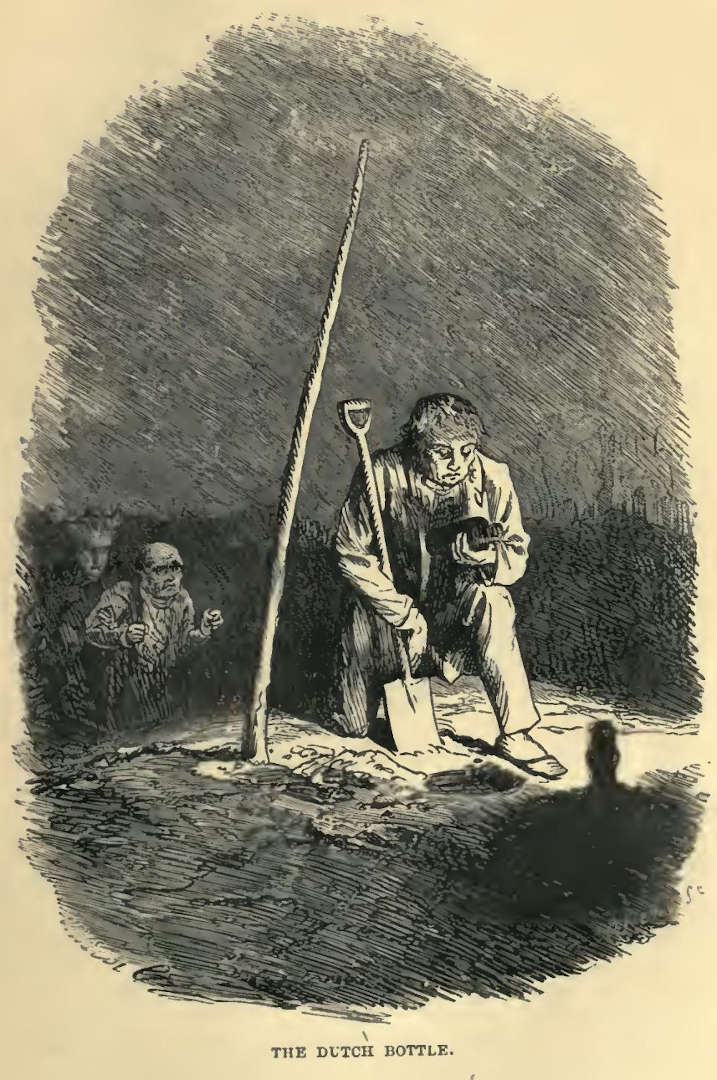
\includegraphics[scale=2.3]{03-06-01}

Mr Boffin came down leisurely, for this brushing process had been well
accomplished, and Mr Venus had had time to take his breath, before he
reappeared. That he had the bottle somewhere about him could not be
doubted; where, was not so clear. He wore a large rough coat, buttoned
over, and it might be in any one of half a dozen pockets.

‘What’s the matter, Wegg?’ said Mr Boffin. ‘You are as pale as a
candle.’

Mr Wegg replied, with literal exactness, that he felt as if he had had a
turn.

‘Bile,’ said Mr Boffin, blowing out the light in the lantern, shutting
it up, and stowing it away in the breast of his coat as before. ‘Are you
subject to bile, Wegg?’

Mr Wegg again replied, with strict adherence to truth, that he didn’t
think he had ever had a similar sensation in his head, to anything like
the same extent.

‘Physic yourself to-morrow, Wegg,’ said Mr Boffin, ‘to be in order
for next night. By-the-by, this neighbourhood is going to have a loss,
Wegg.’

‘A loss, sir?’

‘Going to lose the Mounds.’

The friendly movers made such an obvious effort not to look at one
another, that they might as well have stared at one another with all
their might.

‘Have you parted with them, Mr Boffin?’ asked Silas.

‘Yes; they’re going. Mine’s as good as gone already.’

‘You mean the little one of the three, with the pole atop, sir.’

‘Yes,’ said Mr Boffin, rubbing his ear in his old way, with that new
touch of craftiness added to it. ‘It has fetched a penny. It’ll begin to
be carted off to-morrow.’

‘Have you been out to take leave of your old friend, sir?’ asked Silas,
jocosely.

‘No,’ said Mr Boffin. ‘What the devil put that in your head?’

He was so sudden and rough, that Wegg, who had been hovering closer
and closer to his skirts, despatching the back of his hand on exploring
expeditions in search of the bottle’s surface, retired two or three
paces.

‘No offence, sir,’ said Wegg, humbly. ‘No offence.’

Mr Boffin eyed him as a dog might eye another dog who wanted his bone;
and actually retorted with a low growl, as the dog might have retorted.

‘Good-night,’ he said, after having sunk into a moody silence, with
his hands clasped behind him, and his eyes suspiciously wandering about
Wegg.--‘No! stop there. I know the way out, and I want no light.’

Avarice, and the evening’s legends of avarice, and the inflammatory
effect of what he had seen, and perhaps the rush of his ill-conditioned
blood to his brain in his descent, wrought Silas Wegg to such a pitch of
insatiable appetite, that when the door closed he made a swoop at it and
drew Venus along with him.

‘He mustn’t go,’ he cried. ‘We mustn’t let him go? He has got that
bottle about him. We must have that bottle.’

‘Why, you wouldn’t take it by force?’ said Venus, restraining him.

‘Wouldn’t I? Yes I would. I’d take it by any force, I’d have it at any
price! Are you so afraid of one old man as to let him go, you coward?’

‘I am so afraid of you, as not to let YOU go,’ muttered Venus, sturdily,
clasping him in his arms.

‘Did you hear him?’ retorted Wegg. ‘Did you hear him say that he was
resolved to disappoint us? Did you hear him say, you cur, that he was
going to have the Mounds cleared off, when no doubt the whole place will
be rummaged? If you haven’t the spirit of a mouse to defend your rights,
I have. Let me go after him.’

As in his wildness he was making a strong struggle for it, Mr Venus
deemed it expedient to lift him, throw him, and fall with him; well
knowing that, once down, he would not be up again easily with his wooden
leg. So they both rolled on the floor, and, as they did so, Mr Boffin
shut the gate.



